\documentclass[14pt]{extarticle}
\usepackage{fontspec}
\usepackage{polyglossia}
\usepackage{amsmath}
\usepackage{amssymb}
\usepackage{xcolor}
\usepackage{fancyhdr}
\usepackage{graphicx}
\usepackage{listings}
\usepackage[most]{tcolorbox}
% \usepackage{setspace}
\usepackage{pifont}
\usepackage{enumitem}
\usepackage{titlesec}
\usepackage[bottom]{footmisc}
\usepackage{titling}
\usepackage{minted}
\usepackage{etoolbox}
\usepackage{array}
\usepackage{extsizes}
\usepackage{float}
\usepackage{booktabs}
\usepackage{hyperref}
\usepackage[onehalfspacing]{setspace}
\usepackage[a4paper, top=2.7cm, bottom=2.7cm, left=2.5cm, right=2.5cm, headheight=1.5cm, headsep=0.5cm]{geometry}
\usepackage{tikz}

\usetikzlibrary{automata, positioning, arrows.meta, arrows}

\newfontfamily\emoji{Segoe UI Emoji}

\pagestyle{fancy}

\setmainlanguage[numerals=western]{arabic}
\setotherlanguage{english}
% \newfontfamily\arabicfont[Script=Arabic]{Amiri}
\newfontfamily\arabicfont[Script=Arabic]{Calibri}
\newfontfamily\arabicfonttt[Script=Arabic]{Courier New}

\lstset{
  language=[Sharp]C,
  numbers=left,
  stepnumber=1,
  numbersep=8pt,
  frame=single,
  basicstyle=\ttfamily\small,
  keywordstyle=\color{blue},
  stringstyle=\color{red},
  commentstyle=\color{green!50!black}
}

\newif\ifdetailed
\ifdefined\setdetailed
  \setdetailed
\fi

\newif\ifwithsols
\ifdefined\setwithsols
  \setwithsols
\fi

% unified tcolorboxes for articles
\tcbset{colback=white, colframe=black, fonttitle=\bfseries, boxrule=0.8pt}
\newtcolorbox{boxDef}[1][]{colback=blue!5!white,colframe=blue!75!black,
  title={{\emoji📘} تعريف\ifx\\#1\\\else ~#1\fi :}}
\newtcolorbox{boxExercise}[1][]{colback=cyan!5!white,colframe=cyan!70!black,
  title={{\emoji🧩} تمرين\ifx\\#1\\\else ~#1\fi :}}
\newtcolorbox{boxExample}[1][]{colback=yellow!5!white,colframe=orange!90!black,
  title={{\emoji📝} مثال\ifx\\#1\\\else ~#1\fi :}}
\newtcolorbox{boxNote}[1][]{colback=gray!10!white,colframe=black,
  title={{\emoji✨} ملاحظة\ifx\\#1\\\else ~#1\fi :}}
\newtcolorbox{boxAttention}[1][]{colback=magenta!10!white,colframe=magenta!80!black,
  title={{\emoji🔔} تنبيه\ifx\\#1\\\else ~#1\fi :}}
\newtcolorbox{boxWarning}[1][]{colback=red!5!white,colframe=red!75!black,
  title={{\emoji⚡} ملاحظة هامة\ifx\\#1\\\else ~#1\fi :}}
\newtcolorbox{boxSolution}[1][]{colback=green!5!white,colframe=green!60!black,
  title={{\emoji✅} حل\ifx\\#1\\\else ~#1\fi :}}
\newtcolorbox{boxSymbol}[1][]{colback=purple!5!white,colframe=purple!70!black,
  title={{\emoji🔣} رمز\ifx\\#1\\\else ~#1\fi :}}
\newtcolorbox{boxHint}[1][]{colback=teal!5!white,colframe=teal!60!black,
  title={{\emoji💡} تلميح\ifx\\#1\\\else ~#1\fi :}}


\tcbset{simplecode/.style={ colback=gray!5, colframe=black!50, boxrule=0.4pt, arc=2pt, left=4pt,right=4pt,top=4pt,bottom=4pt}}
\newenvironment{boxCode}{\begin{tcolorbox}[simplecode]}{\end{tcolorbox}}

\newcolumntype{C}[1]{>{\centering\arraybackslash}p{#1}}

% redefine spaces after titles
\makeatletter
\renewcommand{\@maketitle}{%
  \begin{center}
    {\huge \bfseries \@title \par}%
    \vskip 0.2em % space between title and author
    {\large \@author \par}%
    % \vskip 0.2em % space between author and date
    % {\normalsize \@date \par}%
  \end{center}
}
\makeatother

\fancyhf{} % clear default
\fancypagestyle{plain}{
  \fancyhf{}
  \fancyhead[L]{مدرسة التسامح الشاملة}
  % \fancyhead[L]{
\includegraphics[height=1cm]{../../../images/logoTasamoh.png}}
  \fancyhead[R]{الأستاذ محمود اغبارية}
  \fancyfoot[C]{\thepage}
}

\fancyhead[L]{مدرسة التسامح الشاملة}
\fancyhead[R]{الأستاذ محمود اغبارية}
\fancyfoot[C]{\thepage}
% \date{\today}

\setcounter{tocdepth}{3} % only section subsection and subsubsection in TOC

\newcommand{\importpdfpage}[2]{%
    \thispagestyle{empty}
    \newgeometry{left=0cm,right=0cm,top=0cm,bottom=0cm}
    \includegraphics[page=#2,width=0.95\paperwidth,height=0.95\paperheight,keepaspectratio]{#1}
    \restoregeometry
}

\newcommand{\insertFullImg}[1]{%
    \noindent
    \makebox[\textwidth][c]{
        \includegraphics[width=0.9\paperwidth,keepaspectratio]{#1}%
    }%
}%

% ----------------------


% \begin{document}

% \maketitle

% % \clearpage  % start TOC on a new page
% % \renewcommand{\contentsname}{جدول المحتويات}
% % \tableofcontents
% % \clearpage

% \part*{part 1} % the * prevents numbering
% \section*{مقدمة}
% \subsection*{مثال رياضي}
% \subsubsection*{مثال فرعي}
% \paragraph*{ paragraph 1}
% \subparagraph*{sub paragraph 1}

% \ifdetailed
% \begin{english}
% \begin{minted}{csharp}
% // C# Example
% \end{minted}
% \end{english}
% \fi

% OLD WAY
% \ifdetailed
% \begin{english}
% \begin{lstlisting}
% // C# Example
% \end{lstlisting}
% \end{english}
% \fi

% % 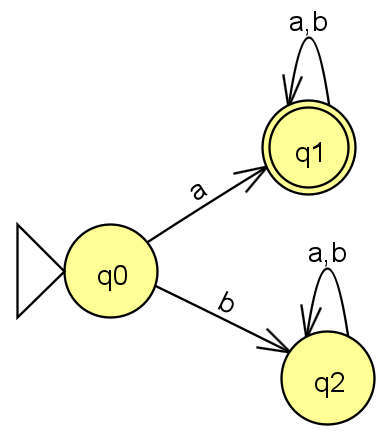
\includegraphics[width=0.2\textwidth]{../../../images/DFAs/ex1_q1.png}



% \vspace{3cm}
% \begin{flushleft}
% أرجو لكم وقتًا ممتعًا.

% الأستاذ محمود اغبارية.
% \end{flushleft}


% \end{document}


\ifwithsols
\title{حل ورقة تمرّن 12 – المصفوفة ثنائية الأبعاد: تدريب شامل}
\else
\title{ورقة تمرّن 12 – المصفوفة ثنائية الأبعاد: تدريب شامل}
\fi

\begin{document}

\maketitle
\thispagestyle{fancy}

نعمل في جميع الأسئلة على المصفوفة \textenglish{mat} التالية ما لم يُذكر خلاف ذلك:

\begin{center}
\begin{english}
\begin{tabular}{c|ccccc}
 & \textbf{[,0]} & \textbf{[,1]} & \textbf{[,2]} & \textbf{[,3]} & \textbf{[,4]} \\
\hline
\textbf{[0,]} &  3 &  7 & -2 &  5 &  1 \\
\textbf{[1,]} &  6 &  4 &  8 &  2 & 10 \\
\textbf{[2,]} & -1 &  9 &  0 &  3 & -4 \\
\textbf{[3,]} &  5 &  2 &  6 & 11 &  3 \\
\end{tabular}
\end{english}
\end{center}

% ════════════════════════════════════════════════════════════
\section*{القسم الأول: أساسيات — الصف والعمود}
% ════════════════════════════════════════════════════════════

\begin{enumerate}[itemsep=2em]

% ----------------------------------------------------------------
\item
اكتب عملية خارجية \textenglish{PrintRow} تتلقى مصفوفة أعداد صحيحة ثنائية الأبعاد \textenglish{mat} وعدداً \textenglish{r}، وتطبع جميع عناصر الصف \textenglish{r} بالترتيب.

\begin{boxExample}
\textenglish{PrintRow(mat, 1)} تطبع: \textenglish{6  4  8  2  10}
\end{boxExample}

\ifwithsols
\begin{boxSolution}
\begin{boxCode}
\begin{english}
\begin{minted}{csharp}
public static void PrintRow(int[,] mat, int r)
{
    for (int j = 0; j < mat.GetLength(1); j++)
        Console.Write(mat[r, j] + "  ");
    Console.WriteLine();
}
\end{minted}
\end{english}
\end{boxCode}
\textbf{الشرح:} نُثبَّت الصف \textenglish{r} ونُغيّر العمود \textenglish{j} من 0 حتى عدد الأعمدة.
\end{boxSolution}
\clearpage
\fi

% ----------------------------------------------------------------
\item
اكتب عملية خارجية \textenglish{PrintCol} تتلقى مصفوفة أعداد صحيحة ثنائية الأبعاد \textenglish{mat} وعدداً \textenglish{c}، وتطبع جميع عناصر العمود \textenglish{c} بالترتيب من الأعلى إلى الأسفل.

\begin{boxExample}
\textenglish{PrintCol(mat, 2)} تطبع: \textenglish{-2}، \textenglish{8}، \textenglish{0}، \textenglish{6}
\end{boxExample}

\ifwithsols
\begin{boxSolution}
\begin{boxCode}
\begin{english}
\begin{minted}{csharp}
public static void PrintCol(int[,] mat, int c)
{
    for (int i = 0; i < mat.GetLength(0); i++)
        Console.WriteLine(mat[i, c]);
}
\end{minted}
\end{english}
\end{boxCode}
\textbf{الشرح:} نُثبَّت العمود \textenglish{c} ونُغيّر الصف \textenglish{i}. الفرق الوحيد عن \textenglish{PrintRow}: أيّ المؤشرين يُثبَّت وأيّهما يتغير.
\end{boxSolution}
\clearpage
\fi

% ----------------------------------------------------------------
\item
اكتب عملية خارجية \textenglish{RowSum} تتلقى مصفوفة أعداد صحيحة ثنائية الأبعاد \textenglish{mat} وعدداً \textenglish{r}، وتُعيد مجموع عناصر الصف \textenglish{r}.

\begin{boxExample}
\textenglish{RowSum(mat, 3)} تُعيد $5+2+6+11+3 = 27$
\end{boxExample}

\ifwithsols
\begin{boxSolution}
\begin{boxCode}
\begin{english}
\begin{minted}{csharp}
public static int RowSum(int[,] mat, int r)
{
    int sum = 0;
    for (int j = 0; j < mat.GetLength(1); j++)
        sum += mat[r, j];
    return sum;
}
\end{minted}
\end{english}
\end{boxCode}
\textbf{الشرح:} نُثبَّت \textenglish{r} ونجمع على \textenglish{j}.
\end{boxSolution}
\clearpage
\fi

% ----------------------------------------------------------------
\item
اكتب عملية خارجية \textenglish{ColMax} تتلقى مصفوفة أعداد صحيحة ثنائية الأبعاد \textenglish{mat} وعدداً \textenglish{c}، وتُعيد أكبر قيمة في العمود \textenglish{c}.

\begin{boxExample}
\textenglish{ColMax(mat, 1)} تُعيد \textenglish{9} (لأن العمود 1 يحتوي: 7، 4، 9، 2)
\end{boxExample}

\ifwithsols
\begin{boxSolution}
\begin{boxCode}
\begin{english}
\begin{minted}{csharp}
public static int ColMax(int[,] mat, int c)
{
    int max = mat[0, c];
    for (int i = 1; i < mat.GetLength(0); i++)
        if (mat[i, c] > max)
            max = mat[i, c];
    return max;
}
\end{minted}
\end{english}
\end{boxCode}
\textbf{الشرح:} نبدأ بافتراض أن أول عنصر في العمود هو الأكبر، ثم نمر على الباقين ونحدّث \textenglish{max}.
\end{boxSolution}
\clearpage
\fi

% ----------------------------------------------------------------
\item
اكتب عملية خارجية \textenglish{IsAllPositiveRow} تتلقى مصفوفة أعداد صحيحة ثنائية الأبعاد \textenglish{mat} وعدداً \textenglish{r}، وتُعيد \textenglish{true} إذا كانت جميع عناصر الصف \textenglish{r} أكبر من صفر.

\begin{boxExample}
\begin{itemize}[itemsep=1pt]
    \item \textenglish{IsAllPositiveRow(mat, 1)} تُعيد \textenglish{true} (كل عناصره: 6، 4، 8، 2، 10 — جميعها موجبة)
    \item \textenglish{IsAllPositiveRow(mat, 0)} تُعيد \textenglish{false} (يحتوي \textenglish{-2})
\end{itemize}
\end{boxExample}

\ifwithsols
\begin{boxSolution}
\begin{boxCode}
\begin{english}
\begin{minted}{csharp}
public static bool IsAllPositiveRow(int[,] mat, int r)
{
    for (int j = 0; j < mat.GetLength(1); j++)
        if (mat[r, j] <= 0)
            return false;
    return true;
}
\end{minted}
\end{english}
\end{boxCode}
\textbf{الشرح:} حالما نجد عنصراً غير موجب نُعيد \textenglish{false} فوراً. إذا انتهت الحلقة بدون ذلك نُعيد \textenglish{true}.
\end{boxSolution}
\fi

\end{enumerate}

% ════════════════════════════════════════════════════════════
\clearpage
\section*{القسم الثاني: مسح المصفوفة كاملةً — خصائص الصفوف والأعمدة}
% ════════════════════════════════════════════════════════════

\begin{enumerate}[itemsep=2em]

% ----------------------------------------------------------------
\item
اكتب عملية خارجية \textenglish{MaxColSum} تتلقى مصفوفة أعداد صحيحة ثنائية الأبعاد \textenglish{mat}، وتُعيد \textbf{رقم العمود} الذي يملك أكبر مجموع.

\begin{boxExample}
في المصفوفة \textenglish{mat} أعلاه:
\begin{itemize}[itemsep=1pt]
    \item مجموع العمود 0: $3+6-1+5=13$
    \item مجموع العمود 1: $7+4+9+2=22$
    \item مجموع العمود 2: $-2+8+0+6=12$
    \item مجموع العمود 3: $5+2+3+11=21$
    \item مجموع العمود 4: $1+10-4+3=10$
\end{itemize}
النتيجة: \textenglish{1} (العمود 1 مجموعه 22 وهو الأكبر)
\end{boxExample}

\begin{boxHint}
يمكنك استخدام عملية مساعدة لحساب مجموع عمود معين.
\end{boxHint}

\ifwithsols
\begin{boxSolution}
\begin{boxCode}
\begin{english}
\begin{minted}{csharp}
public static int ColSum(int[,] mat, int c)
{
    int sum = 0;
    for (int i = 0; i < mat.GetLength(0); i++)
        sum += mat[i, c];
    return sum;
}

public static int MaxColSum(int[,] mat)
{
    int maxIdx = 0;
    int maxSum = ColSum(mat, 0);
    for (int j = 1; j < mat.GetLength(1); j++)
    {
        int s = ColSum(mat, j);
        if (s > maxSum)
        {
            maxSum = s;
            maxIdx = j;
        }
    }
    return maxIdx;
}
\end{minted}
\end{english}
\end{boxCode}
\textbf{الشرح:} نحسب مجموع كل عمود ونقارنه بأكبر مجموع رأيناه حتى الآن. نحتفظ بـ\textenglish{maxIdx} لأن السؤال يطلب رقم العمود لا مجموعه.
\end{boxSolution}
\clearpage
\fi

% ----------------------------------------------------------------
\item
اكتب عملية خارجية \textenglish{CountRowsAbove} تتلقى مصفوفة أعداد صحيحة ثنائية الأبعاد \textenglish{mat} وعدداً \textenglish{threshold}، وتُعيد عدد الصفوف التي مجموعها \textbf{أكبر تماماً} من \textenglish{threshold}.

\begin{boxExample}
\textenglish{CountRowsAbove(mat, 20)}:
\begin{itemize}[itemsep=1pt]
    \item مجموع الصف 0: $3+7-2+5+1=14$ — لا
    \item مجموع الصف 1: $6+4+8+2+10=30$ — نعم
    \item مجموع الصف 2: $-1+9+0+3-4=7$ — لا
    \item مجموع الصف 3: $5+2+6+11+3=27$ — نعم
\end{itemize}
النتيجة: \textenglish{2}
\end{boxExample}

\ifwithsols
\begin{boxSolution}
\begin{boxCode}
\begin{english}
\begin{minted}{csharp}
public static int CountRowsAbove(int[,] mat, int threshold)
{
    int count = 0;
    for (int i = 0; i < mat.GetLength(0); i++)
    {
        int sum = 0;
        for (int j = 0; j < mat.GetLength(1); j++)
            sum += mat[i, j];
        if (sum > threshold)
            count++;
    }
    return count;
}
\end{minted}
\end{english}
\end{boxCode}
\textbf{الشرح:} في كل دورة \textenglish{i} نحسب مجموع الصف الحالي بحلقة داخلية، ثم نفحص هل يتجاوز \textenglish{threshold}.
\end{boxSolution}
\clearpage
\fi

% ----------------------------------------------------------------
\item
اكتب عملية خارجية \textenglish{AreColsEqual} تتلقى مصفوفة أعداد صحيحة ثنائية الأبعاد \textenglish{mat} ورقمَي عمودَين \textenglish{c1} و\textenglish{c2}، وتُعيد \textenglish{true} إذا كان العمودان يحتويان على نفس القيم بنفس الترتيب.

\begin{boxExample}
في المصفوفة \textenglish{\{\{1,3,1\},\{2,5,2\},\{4,7,4\}\}}:
\begin{itemize}[itemsep=1pt]
    \item \textenglish{AreColsEqual(mat, 0, 2)} تُعيد \textenglish{true}
    \item \textenglish{AreColsEqual(mat, 0, 1)} تُعيد \textenglish{false}
\end{itemize}
\end{boxExample}

\ifwithsols
\begin{boxSolution}
\begin{boxCode}
\begin{english}
\begin{minted}{csharp}
public static bool AreColsEqual(int[,] mat, int c1, int c2)
{
    for (int i = 0; i < mat.GetLength(0); i++)
        if (mat[i, c1] != mat[i, c2])
            return false;
    return true;
}
\end{minted}
\end{english}
\end{boxCode}
\textbf{الشرح:} نقارن عناصر العمودَين عنصراً عنصراً في نفس الصف. نمط "حالما نجد اختلافاً نُعيد \textenglish{false}" يُجنّبنا المرور الزائد.
\end{boxSolution}
\clearpage
\fi

% ----------------------------------------------------------------
\item
اكتب عملية خارجية \textenglish{HasEqualCols} تتلقى مصفوفة أعداد صحيحة ثنائية الأبعاد \textenglish{mat}، وتُعيد \textenglish{true} إذا وُجد في المصفوفة عمودان (أو أكثر) متطابقان، و\textenglish{false} في غير ذلك.

\begin{boxHint}
يمكنك استخدام \textenglish{AreColsEqual} من السؤال السابق.
\end{boxHint}

\ifwithsols
\begin{boxSolution}
\begin{boxCode}
\begin{english}
\begin{minted}{csharp}
public static bool HasEqualCols(int[,] mat)
{
    int cols = mat.GetLength(1);
    for (int c1 = 0; c1 < cols - 1; c1++)
        for (int c2 = c1 + 1; c2 < cols; c2++)
            if (AreColsEqual(mat, c1, c2))
                return true;
    return false;
}
\end{minted}
\end{english}
\end{boxCode}
\textbf{الشرح:} نفحص كل زوج من الأعمدة مرة واحدة فقط (\textenglish{c2} يبدأ من \textenglish{c1+1} لتجنب التكرار). حالما نجد زوجاً متطابقاً نُعيد \textenglish{true}.
\end{boxSolution}
\fi

\end{enumerate}

% ════════════════════════════════════════════════════════════
\clearpage
\section*{القسم الثالث: خصائص الموضع (i,j) والجوار}
% ════════════════════════════════════════════════════════════

\begin{enumerate}[itemsep=2em]

% ----------------------------------------------------------------
\item
\textbf{يُدعى حدٌّ "محلياً أكبر"} إذا كانت قيمته أكبر من قيم جميع جيرانه الأربعة (أعلى، أسفل، يسار، يمين) الموجودين فيه.

اكتب عملية خارجية \textenglish{IsLocalMax} تتلقى مصفوفة أعداد صحيحة ثنائية الأبعاد \textenglish{mat} وعددَين \textenglish{row} و\textenglish{col}، وتُعيد \textenglish{true} إذا كان \textenglish{mat[row,col]} محلياً أكبر.

\begin{boxExample}
في المصفوفة \textenglish{mat} أعلاه:
\begin{itemize}[itemsep=1pt]
    \item \textenglish{IsLocalMax(mat, 1, 2)}: قيمته 8. جيرانه: \textenglish{-2} (أعلى)، \textenglish{0} (أسفل)، \textenglish{4} (يسار)، \textenglish{2} (يمين). 8 أكبر من جميعهم. النتيجة \textenglish{true}.
    \item \textenglish{IsLocalMax(mat, 3, 3)}: قيمته 11. جيرانه: \textenglish{2} (يسار)، \textenglish{3} (يمين)، \textenglish{2} (أعلى). (أسفل غير موجود — على الحافة). 11 أكبر من جميع جيرانه الموجودين. النتيجة \textenglish{true}.
\end{itemize}
\end{boxExample}

\ifwithsols
\begin{boxSolution}
\begin{boxCode}
\begin{english}
\begin{minted}{csharp}
public static bool IsLocalMax(int[,] mat, int row, int col)
{
    int val = mat[row, col];
    int rows = mat.GetLength(0);
    int cols = mat.GetLength(1);

    if (row > 0       && mat[row-1, col] >= val) return false;
    if (row < rows-1  && mat[row+1, col] >= val) return false;
    if (col > 0       && mat[row, col-1] >= val) return false;
    if (col < cols-1  && mat[row, col+1] >= val) return false;

    return true;
}
\end{minted}
\end{english}
\end{boxCode}
\textbf{الشرح:} لكل جار: نفحص أولاً أنه موجود (ضمن الحدود)، ثم إذا كان قيمته $\geq$ قيمة العنصر الحالي نُعيد \textenglish{false} فوراً. إذا اجتاز العنصر جميع الفحوصات نُعيد \textenglish{true}.
\end{boxSolution}
\clearpage
\fi

% ----------------------------------------------------------------
\item
اكتب عملية خارجية \textenglish{CountLocalMax} تتلقى مصفوفة أعداد صحيحة ثنائية الأبعاد \textenglish{mat}، وتُعيد عدد الحدود المحلية الأكبر فيها.

\begin{boxHint}
استخدم \textenglish{IsLocalMax} من السؤال السابق.
\end{boxHint}

\ifwithsols
\begin{boxSolution}
\begin{boxCode}
\begin{english}
\begin{minted}{csharp}
public static int CountLocalMax(int[,] mat)
{
    int count = 0;
    for (int i = 0; i < mat.GetLength(0); i++)
        for (int j = 0; j < mat.GetLength(1); j++)
            if (IsLocalMax(mat, i, j))
                count++;
    return count;
}
\end{minted}
\end{english}
\end{boxCode}
\textbf{الشرح:} نمط "مرور كامل + عدّ العناصر التي تحقق خاصية" — يتكرر كثيراً في البجروت.
\end{boxSolution}
\fi

\clearpage
% ----------------------------------------------------------------
\item
\textbf{يُدعى حدٌّ "متوازناً"} إذا كان مجموع الحدود \textbf{فوقه في نفس العمود} (من الصف 0 حتى الصف الذي فوقه مباشرةً) يساوي مجموع الحدود \textbf{تحته في نفس العمود} (من الصف الذي تحته مباشرةً حتى آخر صف).

\begin{boxExample}
في العمود 3 من المصفوفة \textenglish{mat}: \textenglish{5، 2، 3، 11}.
فحص الحدّ \textenglish{[1,3]=2}: مجموع ما فوقه = \textenglish{5}، مجموع ما تحته = $3+11=14$. غير متوازن.
فحص الحدّ \textenglish{[2,3]=3}: مجموع ما فوقه = $5+2=7$، مجموع ما تحته = \textenglish{11}. غير متوازن.
\end{boxExample}

اكتب عملية خارجية \textenglish{IsBalanced} تتلقى مصفوفة أعداد صحيحة ثنائية الأبعاد \textenglish{mat} وعددَين \textenglish{row} و\textenglish{col}، وتُعيد \textenglish{true} إذا كان الحدّ \textenglish{mat[row,col]} متوازناً.

\ifwithsols
\begin{boxSolution}
\begin{boxCode}
\begin{english}
\begin{minted}{csharp}
public static bool IsBalanced(int[,] mat, int row, int col)
{
    int above = 0;
    for (int i = 0; i < row; i++)
        above += mat[i, col];

    int below = 0;
    for (int i = row + 1; i < mat.GetLength(0); i++)
        below += mat[i, col];

    return above == below;
}
\end{minted}
\end{english}
\end{boxCode}
\textbf{الشرح:} حلقتان منفصلتان في نفس العمود — الأولى من 0 حتى \textenglish{row-1}، والثانية من \textenglish{row+1} حتى النهاية. الحدّ نفسه (\textenglish{row}) مُستثنى من كليهما.
\end{boxSolution}
\fi

\end{enumerate}

% ════════════════════════════════════════════════════════════
\clearpage
\section*{القسم الرابع: المصفوفة الفرعية (النافذة)}
% ════════════════════════════════════════════════════════════

\begin{boxDef}
\textbf{المصفوفة الفرعية} بكبَر $n \times n$ التي تبدأ في المكان \textenglish{[k,j]} هي مجموعة العناصر:
\textenglish{mat[k..k+n-1, j..j+n-1]} — أي مربع عرضه \textenglish{n} وارتفاعه \textenglish{n} يبدأ من الزاوية \textenglish{[k,j]}.
\end{boxDef}

\begin{enumerate}[itemsep=2em]

% ----------------------------------------------------------------
\item
اكتب عملية خارجية \textenglish{SubMatSum} تتلقى مصفوفة أعداد صحيحة ثنائية الأبعاد \textenglish{mat} وثلاثة أعداد \textenglish{k}، \textenglish{j}، \textenglish{n}، وتُعيد مجموع عناصر المصفوفة الفرعية $n\times n$ التي تبدأ في \textenglish{[k,j]}.

\begin{boxExample}
\textenglish{SubMatSum(mat, 0, 1, 3)} تُعيد مجموع العناصر:
\begin{center}
\begin{english}
\begin{tabular}{|c|c|c|}
\hline
7 & -2 & 5 \\
\hline
4 &  8 & 2 \\
\hline
9 &  0 & 3 \\
\hline
\end{tabular}
\end{english}
\end{center}
$7-2+5+4+8+2+9+0+3 = 36$
\end{boxExample}

\ifwithsols
\begin{boxSolution}
\begin{boxCode}
\begin{english}
\begin{minted}{csharp}
public static int SubMatSum(int[,] mat, int k, int j, int n)
{
    int sum = 0;
    for (int i = k; i < k + n; i++)
        for (int jj = j; jj < j + n; jj++)
            sum += mat[i, jj];
    return sum;
}
\end{minted}
\end{english}
\end{boxCode}
\textbf{الشرح:} الحلقتان تبدآن من \textenglish{k} وـ\textenglish{j} وتنتهيان بعد \textenglish{n} خطوات بدلاً من نهاية المصفوفة كاملةً.
\end{boxSolution}
\clearpage
\fi

% ----------------------------------------------------------------
\item
\textbf{تُسمّى مصفوفة فرعية $2\times2$ "متجانسة"} إذا كانت جميع عناصرها متساوية.

اكتب عملية خارجية \textenglish{IsUniform2x2} تتلقى مصفوفة أعداد صحيحة ثنائية الأبعاد \textenglish{mat} وعددَين \textenglish{k}، \textenglish{j}، وتُعيد \textenglish{true} إذا كانت المصفوفة الفرعية $2\times2$ التي تبدأ في \textenglish{[k,j]} متجانسة.

ثم اكتب عملية خارجية \textenglish{CountUniform2x2} تتلقى مصفوفة \textenglish{mat} وتُعيد عدد المصفوفات الفرعية $2\times2$ المتجانسة فيها.

\begin{boxExample}
في المصفوفة \textenglish{\{\{3,3,1\},\{3,3,2\},\{4,5,6\}\}}: توجد مصفوفة فرعية متجانسة واحدة تبدأ في \textenglish{[0,0]} (كلها 3).
\end{boxExample}

\ifwithsols
\begin{boxSolution}
\begin{boxCode}
\begin{english}
\begin{minted}{csharp}
public static bool IsUniform2x2(int[,] mat, int k, int j)
{
    int val = mat[k, j];
    return mat[k,   j+1] == val &&
           mat[k+1, j  ] == val &&
           mat[k+1, j+1] == val;
}

public static int CountUniform2x2(int[,] mat)
{
    int count = 0;
    for (int i = 0; i <= mat.GetLength(0) - 2; i++)
        for (int j = 0; j <= mat.GetLength(1) - 2; j++)
            if (IsUniform2x2(mat, i, j))
                count++;
    return count;
}
\end{minted}
\end{english}
\end{boxCode}
\textbf{الشرح:} في \textenglish{IsUniform2x2} نقارن الثلاثة عناصر الأخرى بالأول. الحلقتان في \textenglish{CountUniform2x2} تتوقفان عند \textenglish{rows-2} وـ\textenglish{cols-2} لأن النافذة تحتاج صفَّين وعمودَين ابتداءً من الموضع الحالي.
\end{boxSolution}
\fi

\clearpage
% ----------------------------------------------------------------
\item
\textbf{تُسمّى مصفوفة فرعية $3\times3$ "متصاعدة"} إذا كانت قيمة زاويتها العليا اليُسرى أصغر من قيمة زاويتها السفلى اليُمنى.

اكتب عملية خارجية \textenglish{IsAscending3x3} تتلقى مصفوفة أعداد صحيحة ثنائية الأبعاد \textenglish{mat} وعددَين \textenglish{k}، \textenglish{j}، وتُعيد \textenglish{true} إذا كانت المصفوفة الفرعية $3\times3$ التي تبدأ في \textenglish{[k,j]} متصاعدة.

ثم اكتب برنامجاً يطبع عدد المصفوفات الفرعية $3\times3$ المتصاعدة في مصفوفة \textenglish{arr} بكبَر $20\times20$.

\ifwithsols
\begin{boxSolution}
\begin{boxCode}
\begin{english}
\begin{minted}{csharp}
public static bool IsAscending3x3(int[,] mat, int k, int j)
{
    return mat[k, j] < mat[k + 2, j + 2];
}

static void Main()
{
    int[,] arr = new int[20, 20];
    // (نفترض أن arr مُعبّأة)

    int count = 0;
    for (int i = 0; i <= 20 - 3; i++)
        for (int j = 0; j <= 20 - 3; j++)
            if (IsAscending3x3(arr, i, j))
                count++;

    Console.WriteLine(count);
}
\end{minted}
\end{english}
\end{boxCode}
\textbf{الشرح:} الزاوية اليُسرى العُليا هي \textenglish{[k,j]}، والزاوية اليُمنى السُفلى هي \textenglish{[k+2,j+2]}. الحلقتان تتوقفان عند \textenglish{rows-3} وـ\textenglish{cols-3}.
\end{boxSolution}
\fi

\end{enumerate}

% ════════════════════════════════════════════════════════════
\clearpage
\section*{القسم الخامس: تعريفات مركّبة — مستوى البجروت}
% ════════════════════════════════════════════════════════════

\begin{boxAttention}
كل سؤال في هذا القسم يتضمن تعريفاً جديداً يجب قراءته بعناية، ثم كتابة عمليتَين: الأولى تفحص خاصية حدٍّ أو نافذة واحدة، والثانية تُطبَّق على المصفوفة كاملةً.
\end{boxAttention}

\begin{enumerate}[itemsep=2em]

% ----------------------------------------------------------------
\item
\textbf{تعريف "حدّ ذروة العمود":} يُسمّى الحدّ \textenglish{mat[i,j]} "ذروة عمود" إذا كانت قيمته أكبر من مجموع جميع العناصر \textbf{الأخرى} في نفس العمود.

\begin{boxExample}
في العمود 1: \textenglish{7، 4، 9، 2}. المجموع الكلي = 22.
\begin{itemize}[itemsep=1pt]
    \item الحدّ 7: مجموع الباقين = $4+9+2=15$. هل $7>15$؟ لا.
    \item الحدّ 9: مجموع الباقين = $7+4+2=13$. هل $9>13$؟ لا.
\end{itemize}
لا يوجد حدّ ذروة عمود في العمود 1.
\end{boxExample}

اكتب:

\textbf{(أ)} عملية \textenglish{IsColPeak} تتلقى مصفوفة \textenglish{mat} وعددَين \textenglish{row}، \textenglish{col}، وتُعيد \textenglish{true} إذا كان \textenglish{mat[row,col]} ذروة عمود.

\textbf{(ب)} عملية \textenglish{CountColPeaks} تتلقى مصفوفة \textenglish{mat} وتُعيد عدد حدود الذروة في جميع أعمدتها.

\ifwithsols
\begin{boxSolution}
\textbf{جزء (أ):}
\begin{boxCode}
\begin{english}
\begin{minted}{csharp}
public static bool IsColPeak(int[,] mat, int row, int col)
{
    int val = mat[row, col];
    int othersSum = 0;
    for (int i = 0; i < mat.GetLength(0); i++)
        if (i != row)
            othersSum += mat[i, col];
    return val > othersSum;
}
\end{minted}
\end{english}
\end{boxCode}

\textbf{جزء (ب):}
\begin{boxCode}
\begin{english}
\begin{minted}{csharp}
public static int CountColPeaks(int[,] mat)
{
    int count = 0;
    for (int i = 0; i < mat.GetLength(0); i++)
        for (int j = 0; j < mat.GetLength(1); j++)
            if (IsColPeak(mat, i, j))
                count++;
    return count;
}
\end{minted}
\end{english}
\end{boxCode}
\textbf{الشرح:} في \textenglish{IsColPeak} نجمع كل عناصر العمود \textenglish{col} \textbf{ما عدا} الصف \textenglish{row} (بالشرط \textenglish{i != row})، ثم نقارن قيمة العنصر بمجموع الباقين.
\end{boxSolution}
\fi

\clearpage
% ----------------------------------------------------------------
\item
\textbf{تعريف "سطر متدرّج":} يُسمّى السطر "متدرجاً تصاعدياً" إذا كانت قيمة كل عنصر فيه أكبر تماماً من قيمة العنصر الذي قبله (من اليسار إلى اليمين).

\begin{boxExample}
في المصفوفة \textenglish{mat} أعلاه:
\begin{itemize}[itemsep=1pt]
    \item الصف 1: \textenglish{6، 4، 8، 2، 10} — \textenglish{4 < 6} ← \textbf{ليس} متدرجاً.
    \item الصف 3: \textenglish{5، 2، 6، 11، 3} — \textenglish{2 < 5} ← \textbf{ليس} متدرجاً.
\end{itemize}
\end{boxExample}

اكتب:

\textbf{(أ)} عملية \textenglish{IsAscendingRow} تتلقى مصفوفة \textenglish{mat} وعدداً \textenglish{r}، وتُعيد \textenglish{true} إذا كان الصف \textenglish{r} متدرجاً تصاعدياً.

\textbf{(ب)} عملية \textenglish{MaxAscendingRowSum} تتلقى مصفوفة \textenglish{mat}، وتُعيد مجموع الصف المتدرج الذي يملك أكبر مجموع. إذا لم يكن هناك صف متدرج تُعيد \textenglish{-1}.

\ifwithsols
\begin{boxSolution}
\textbf{جزء (أ):}
\begin{boxCode}
\begin{english}
\begin{minted}{csharp}
public static bool IsAscendingRow(int[,] mat, int r)
{
    for (int j = 1; j < mat.GetLength(1); j++)
        if (mat[r, j] <= mat[r, j - 1])
            return false;
    return true;
}
\end{minted}
\end{english}
\end{boxCode}

\textbf{جزء (ب):}
\begin{boxCode}
\begin{english}
\begin{minted}{csharp}
public static int MaxAscendingRowSum(int[,] mat)
{
    int maxSum = -1;
    for (int i = 0; i < mat.GetLength(0); i++)
    {
        if (!IsAscendingRow(mat, i))
            continue;
        int s = 0;
        for (int j = 0; j < mat.GetLength(1); j++)
            s += mat[i, j];
        if (s > maxSum)
            maxSum = s;
    }
    return maxSum;
}
\end{minted}
\end{english}
\end{boxCode}
\textbf{الشرح:} في جزء (أ) نقارن كل عنصر بالذي قبله — نبدأ من \textenglish{j=1}. في جزء (ب) نتخطى الصفوف غير المتدرجة بـ\textenglish{continue}، ونحسب مجموع المتدرجة فقط.
\end{boxSolution}
\fi

\clearpage
% ----------------------------------------------------------------
\item
\textbf{تعريف "حدّ مركزي":} في مصفوفة فرعية $3\times3$، يُسمّى العنصر الأوسط \textenglish{mat[k+1,j+1]} "مركزياً" إذا كانت قيمته تساوي متوسط (معدّل) مجموع الحدود الأربعة في زوايا هذه المصفوفة الفرعية.

\begin{boxExample}
المصفوفة الفرعية $3\times3$ التي تبدأ في \textenglish{[1,0]} من \textenglish{mat}:
\begin{center}
\begin{english}
\begin{tabular}{|c|c|c|}
\hline
\textbf{6} & 4 & \textbf{8} \\
\hline
-1 & \textit{9} & 0 \\
\hline
\textbf{5} & 2 & \textbf{6} \\
\hline
\end{tabular}
\end{english}
\end{center}
الزوايا: $6، 8، 5، 6$. مجموعها = 25. متوسطها = $25/4 = 6.25$.
العنصر المركزي = 9. هل $9 = 6.25$؟ لا.
\end{boxExample}

اكتب:

\textbf{(أ)} عملية \textenglish{IsCentral} تتلقى مصفوفة \textenglish{mat} وعددَين \textenglish{k}، \textenglish{j}، وتُعيد \textenglish{true} إذا كان العنصر المركزي للمصفوفة الفرعية $3\times3$ التي تبدأ في \textenglish{[k,j]} مركزياً.

\textbf{(ب)} برنامجاً يعدّ ويطبع عدد العناصر المركزية في مصفوفة \textenglish{arr} بكبَر $15\times18$.

\ifwithsols
\begin{boxSolution}
\textbf{جزء (أ):}
\begin{boxCode}
\begin{english}
\begin{minted}{csharp}
public static bool IsCentral(int[,] mat, int k, int j)
{
    int cornerSum = mat[k,   j  ] + mat[k,   j+2]
                  + mat[k+2, j  ] + mat[k+2, j+2];
    int center = mat[k + 1, j + 1];
    // المقارنة: center == cornerSum / 4.0
    // نتجنب الكسور: center * 4 == cornerSum
    return center * 4 == cornerSum;
}
\end{minted}
\end{english}
\end{boxCode}

\textbf{جزء (ب):}
\begin{boxCode}
\begin{english}
\begin{minted}{csharp}
static void Main()
{
    int[,] arr = new int[15, 18];
    // (نفترض أن arr مُعبّأة)

    int count = 0;
    for (int i = 0; i <= 15 - 3; i++)
        for (int j = 0; j <= 18 - 3; j++)
            if (IsCentral(arr, i, j))
                count++;

    Console.WriteLine(count);
}
\end{minted}
\end{english}
\end{boxCode}
\textbf{الشرح:} الزوايا الأربع للمصفوفة $3\times3$ التي تبدأ في \textenglish{[k,j]} هي: \textenglish{[k,j]}، \textenglish{[k,j+2]}، \textenglish{[k+2,j]}، \textenglish{[k+2,j+2]}. نتجنب قسمة الأعداد الصحيحة بضرب المركز في 4 بدلاً من قسمة المجموع على 4.
\end{boxSolution}
\fi

\end{enumerate}

\vspace{1cm}
\begin{flushleft}
أرجو لكم عملاً ممتعاً!

الأستاذ محمود اغبارية
\end{flushleft}

\end{document}